\chapter{Analyse de domaine}
\begin{preamble}
Dans ce chapitre nous analysons un large éventail de services d'assistance domiciliaire dédié aux personnes âgées, en considérant la variété des besoins des intervenants, pour identifier les concepts clés et les opérations spécifiques pour le traitement de la sensibilité au contexte. Reposant sur cette analyse, nous proposons un langage dédié et sensible au contexte avec son architecture logicielle. Cette approche permet de mettre en synergie les intervenants d'une maison sensible au contexte, en leur fournissant une approche unifiée pour concevoir et développer des services.
\end{preamble}
\chpsummary{Contributions}
{
{\em Analyse de domain} Identification des concepts clés et des opérations spécifiques au traitement sensible au contexte.;
{\em Langage dédié} Un langage spécifique pour développer un large spectre de services sensibles au contexte, avec un haut niveau d'asbtraction et un traitement uniforme de source de données hétérogènes.;
%\myparagraph{Compiler} We have implemented a compiler for our DSL that maps high-level rules into low-level requests, crunched by an event-processing engine.
{\em Validation} re-définition de 55 services, couvrant les besoins de tous les intervenants d'une plate-forme d'assistance pour le maintien à domicile de personnes âgées.
}


La notion de {\em contexte} est fondamentales dans les champ de l'informatique ubiquitaire et englobe de beaucoup de dimensions, le monde physique, un individu, ses activités, les technologies déployées, etc~\cite{bauer2012comparison}.
% This wide range of dimensions is reflected in the host of application areas that leverages context awareness, spanning infrastructures ({\em e.g.,} railways), premises ({\em e.g.,} buildings), and health ({\em e.g.,} physiological status). 
Une attention particulière de la recherche a été portée sur le {\em domicile} ({\em e.g.,}~\cite{cook2013casas,feminella2014piloteur}). Ce périmètre implique beaucoup de dimensions contextuelles, notamment les interactions physiques avec l'environnement ({\em i.e.,} capteurs), les interactions numériques avec l'environnement de l'utilisateur ({\em i.e.,} email, agenda), l'état des nombreux composants de l'infrastructure de l'informatique ubiquitaire (matériel, logiciel et réseau), les préoccupations relatives aux applications ({\em i.e.,} détection d'activité). Concernant la population générale, le défit récurant est d;identifier de quels services ont besoins les utilisateurs~\cite{brush2011home}, et plus généralement, de développer de méthodes pour recueillir et analyser ces besoins~\cite{coutaz2010disqo}.

Toutefois, dans le domaine du maintien à domicile de personne âgées, un tel environnement peut fournir
des services d’assistance pour pallier les pertes cognitives dues au vieillissement et assurer une vie
indépendante({\em e.g.,} ~\cite{rashidi2013survey}). Ces services sont principalement: (1) détecter et rappeler les activités du quotidien ({\em e.g.,} préparation de repas, toilette, se coucher) pour maintenir le status fonctionnel de l'utilisateur~\cite{caroux2014verification} et (2) surveiller les situations potentiellement dangereuses ({\em e.g.,} cuisinière, porte d'entrée) pour garantir la sécurité de l'utilisateur~\cite{rashidi2013survey}. 
Parce qu’elle implique plusieurs disciplines, une maison équipée d’informatique ubiquitaire et
dédiée au maintien à domicile de personnes âgées demande l’implication d’une variété d’intervenants, tant pour concevoir et développer des services d’assistance, que pour déployer et maintenir l’infrastructure sous-jacente. De ce fait parmi ces intervenants on retrouve les personnes âgées elle-même, les aidants, les expets en vieillissement, les professionnels de santé, les développeurs d'applications ainsi que les techniciens de maintenance. 
Cette grande diversité d’intervenants correspond à une diversité
de contextes : les services de chaque intervenant repose sur des contextes spécifiques (état des
capteurs pour la maintenance, utilisation du frigidaire pour l’assistance à domicile). Ces différents
contextes sont généralement étudiés séparément, en silo. Typiquement, chaque intervenant développe sa propre approche, pour extraire ses informations contextuelles, empêchant toute synergie.

Nous avons analysé un large éventail de services d'assistance domiciliaire dédié aux personnes âgées, en considérant la variété des besoins des intervenants. Ces services sont installés sur une plate-forme d'assistance domiciliaire déployée chez 129 personnes âgées vivant seules et âgées de 82 ans en moyenne~\cite{consel2017homeassist}. 
Cette analyse a permis d'identifier les concepts commun et les variations
entre différentes couches de services déployés et utilisés au quotidien,
pour en extraire des concepts clés et des opérations spécifiques aux
traitements sensibles au contexte.

%\subsection*{Our Approach}

Nous basant sur cette analyse, nous proposons un langage de spécifique, sensible au contexte, appelé Maloya et son architecture logiciel, qui fournie un cadre de conception et les outils pour concevoir et développer des services domiciliaires. Pour unifier les source hétérogènes de données, de composants matériels aux composant logiciels, notre approche promeut un paradigme ``centré données'' et ``orienté données''. Notre approche est {\em centrée données} pour fournir une vue canonique des données mesurée à l'ensemble des services, couvrant les services de maintenance requérant l'état bas niveau des capteurs, jusqu'aux services spécifiques aux aidants nécessitants des mesures d'activités de haut niveau. Notre approche est {\em orientée données} avec des services définis en terme de règles traitant des évènements et des états.


To unify the way services are developed, our approach introduces abstractions and notations that are specific to context-aware processing. The resulting {\em domain-specific language} (DSL) covers the needs of the stakeholders and provides an abstraction layer over underlying, well-established concepts and technologies, such as Allen's algebra to express sequences of interactions~\cite{Allen} and complex-event-processing engines to efficiently process the rules generated from DSL services ({\em e.g.,}~\cite{Cugola:2012:PFI:2187671.2187677}). Furthermore, we envision that our language can serve as a high-level stepping stone to introduce end-user programming languages for stakeholders with no computer-programming background.

To validate our approach, we have re-implemented 55 services ranging over all the stakeholders of the assisted living platform under study. These new services were deployed and successfully tested for their effectiveness in performing the specific tasks of the stakeholders: detection of daily activities, detection of user risks, sensor failure, {\em etc.}

% \subsection*{Contributions}
% To summarize, this paper makes the following contributions.

% \myparagraph {Domain analysis} We provide an analysis of context-aware processing layers in the domain of aging in place. From this analysis, we identify key concepts and operations specific to context-aware processing.

% \myparagraph {Domain-specific language} We introduce a language, specific to developing context-aware services, providing high-level abstractions and notations. 
% Underlying this language is a data-centric and data-driven paradigm that allows services from a range of stakeholders to uniformly process heterogeneous sources of sensed data.

% \myparagraph{Compiler} We have implemented a compiler for our DSL that maps high-level rules into low-level requests, crunched by an event-processing engine.

% \myparagraph {Validation} We applied our approach to re-implement 55 services, ranging over all the stakeholders of an assisted living platform dedicated to aging in place. The resulting services are expressed at a high level and are effective in performing the tasks of the stakeholders.





\section{Domain analysis}
La sensibilité au contexte dans le maintien à domicile des personnes âgées reste jeune et le chemin vers l'adoption est encore en étude~\cite{kaye2017making}. La littérature comporte encore peu d'articles concernant le déploiement de solutions d'assistances dans le domicile réel d'utilisateurs ({\em e.g.,} \cite{kaye2011intelligent}). Heureusement, nous avons pu faire levier sur le projet DomAssist pour conduire notre analyse du domaine sur les domiciles sensibles au contexte pour le maintien à domicile des personnes âgées.

\subsection{DomAssist: Un domicile sensible au contexte pour le maintien à domicile des personnes âgées}

DomAssist est une plate-forme d'assistance qui fournit un catalogue d'applications d'assistance, pour le support des activités du quotidien, la sécurité de l'utilisateur et ses interactions sociales~\cite{consel2017homeassist}. DomAssist est déployée les domiciles de 129 personnes vivants seule âgées de 82 ans en moyenne, pour une durée de 12 mois.

DomAssist est un parfait cas d'étude sur lequel construire une approche unifier pour développer des services pour domiciles sensibles au contexte dédié au maintien a domicile. Il rassemble tout les besoins pour viser notre but: (1) il est déployé dans des environnements réels; (2) il supporte le maintien a domicile de personnes âgées avec des utilisateur fragiles et des besoins immédiats; (3) l'étude conduite est suffisamment longue pour que les problèmes de maintenances et d'évolution aient à être traité rigoureusement; (4) la plate-forme est déployée à une échelle suffisamment large pour que l'administration des domiciles sensibles au contexte ait besoin d'être supporté par des services; (5) les services existant reflètent un large éventail de besoins exprimés par les intervenants, couvrant les utilisateurs, les aidants, les ergothérapeutes, les psychologues, les experts en facteurs humains, les techniciens d'installation et de maintenance, et les informaticiens.

Décrivons maintenant la plate-forme pour délimiter la courverture des services sensibles au contexte. DomAssist se compose d'une architecture client-serveur, pour laquelle le serveur instancie autant de machine virtuelle qu'il y a de domicile sensible au contexte. Chaque machine virtuelle exécute les services d'assistance selectionnés par l'utilisateur et ses aidants. Ces services d'assistance sont alimentés par des données envoyées par Internet via une passerelle déployée dans le domicile. Cette passerelle rassemble les informations en provenance des capteurs placés dans des endroits stratégiques pour surveiller les activités. 
 As well, the gateway channels actions from the services to the home's actuators. In the HomeAssist field study, a typical home consists of 4 contact sensors (entrance door, drawers, cabinets, {\em etc.}), 6 motion detectors (entrance area, kitchen, bathroom, {\em etc.}), and 2 smart plugs, which measure the electricity consumption and turn on/off a connected appliance (microwave, light path, coffeemaker, {\em etc.}). The number and type of devices can vary depending on the configuration of the home and the activities to be monitored. Finally, the home is equipped with a stationary tablet, placed at a central location in the home and always connected to a power outlet. This tablet is dedicated to interacting with the user via notifications emitted by assistive applications, which need to alert the user of a given situation ({\em e.g.} unattended entrance door left open)~\cite{consel2015unifying}.

% Let us now illustrate the diversity of issues addressed by HomeAssist with a set of existing scenarios dedicated to support aging in place.




%**********************************************
\subsection{Scénarios pour le maintien à domicile}\label{domain:scenario}
Nous présentons maintenant quatre scénarios illustrant la variété d'intervenants et de préoccupations nécessaires au support du maintien à domicile de personnes âgées à l'aide d'une maison sensible au contexte (voir Figure~\ref{scenario-fig}). Le premier scénario adresse la sécurité de l'utilisateur. Ce scénario surveille la porte d'entrée pour s'assurer qu'elle ne reste pas ouverte trop longtemps sans être surveillée. Le deuxième scénario, se rapporte au besoin de l'aidant en terme de surveillance des activités du quotidien, en particulier, les routines de préparation de repas. Les deux dernier scénarios concernent des besoins exprimés par les techniciens pour garder les domiciles sensible au contexte opérationnels. Le premier scénario de maintenance détecte l'utilisation d'un placard sans que celle-ci soit recouverte par la détection d'une présence. Le second scénario de maintenance détecte quand un capteur échoue à communiquer; cette situation se produit lorsque le capteur n'a plus de batterie ou dysfonctionne.

\begin{figure*}[t]
\begin{tabular}{| l | l | l | p{7cm} |} \hline
{\bf Stakeholder} & {\bf Domain} & {\bf Name} & {\bf Description} \\ \hline \hline
Older adult& Safety & Door Alert & Entrance door \uline{is open} and  \uline{is unattended} \dotuline{for 5 minutes} \\ \hline
Caregiver & \begin{tabular}{ll} Daily \\ Activities \end{tabular} 
       & \begin{tabular}{ll} Reheating \\ A Frozen Meal\end{tabular} 
          & Freezer \dashuline{gets used} and stove \dashuline{gets turned on} \dotuline{within 10 minutes} or Freezer \dashuline{gets used} during stove \uline{is on},
during \uline{lunch time} (or dinner time) \\ \hline
\begin{tabular}{ll} Home \\Technician \end{tabular}
               & Maintenance & \begin{tabular}{ll} Presence \\ Dependency\end{tabular} 
                  & Whenever the cupboard \dashuline{gets opened} in the kitchen, a presence in the kitchen \uline{is true} \\ \hline
\begin{tabular}{ll} Home \\Technician \end{tabular}
   & Maintenance 
        & \begin{tabular}{ll} Communication \\ Failure \end{tabular} 
             & A sensor \uline{fails to communicate} \dotuline{for 24 hours} and its status does not \dashuline{get updated} \\ \hline
\end{tabular}
\caption{Example scenarios for assistive services}
\label{scenario-fig}
\end{figure*}

Ces scénario offre un apperçu sur les type de services sensibles au contexte nécessaire pour supporter le maintien à domicile de personnes âgées. Certains services tels que ``Door Alert'', peuvent convenir à la plupart des utilisateur. En revanche d'autres services, typiquement, les services concernant les activités du quotidien nécessite un certain degrée de personnalisation pour être efficace. Ceci est illustré par l'activité de préparation de repas et le scénario ``Reheating a Frozen Meal''.

De la même manière, ``Communication Failure'' peut s'appliquer à n'importe quel domicile sensible au contexte, alors que ``Presence Dependency'' demande d'instancier les règles en fonction de la localisation des capteurs. 

\subsection{Analyse de commonalités et variabilités}
Pour conduire notre analyse du domaine, nous avons examiné un éventail de services offert par DomAssist pour identifier leurs commonalités et leurs variabilités. Ces services sont développés en Java en utilisant une méthodologie de conception outillée~\cite{bertran2014diasuite,cassou2012toward}.

We now present the outcomes of this analysis that take the form of high-level, domain-specific concepts. These concepts will pave the way to our domain-specific approach presented in the next section.

\myparagraph{Commonalités} Tous les services se réfèrent à une notion d'{\em environnement} à partir duquel effectuer les mesures. Ces mesures englobent les interactions à la fois dans l'environnement physique ({\em e.g.,} un mouvement détecté) et dans l'environnement numérique ({\em e.g.,} un rappel d'évènement délivré par un agenda). De plus, nous avons identifié deux concepts complémentaires associé à l'environnement: évènements et états. D'un côté, un {\em évènement} définie une mesure d'environnement qui change ({\em e.g.,} une porte devient ouverte/fermée) -- les évènements sont soulignés avec des pointillés dans les scénarios de la Figure~\ref{scenario-fig}. D'un autre côté, un {\em état} rend un évènements persistant à travers le temps ({\em e.g.,} la porte {\em est} ouverte) -- les états sous soulignés avec une ligne pleine dans la Figure~\ref{scenario-fig}. Une fois ces concepts identifiés, nous définissons les façons spécifiques de les combiner, exposant les commonalités de {\em composition}. Spécifiquement, la combinaison de mesures d'environnement peut définir un {\em ordre} dans lequel les interaction doivent arriver et leur {\em durée} -- ces contraintes sont soulignées avec des points dans la Figure~\ref{scenario-fig}.

Étudions plus en détail ces points communs en examinant leur spectre de variabilité.

\myparagraph{Variabilités} Les mesures environnementales peuvent être réalisées par une variété d'entités, matérielles ({\em e.g.,} capteurs), logicielles ({\em e.g.,} agenda), locales ({\em e.g.,} porte), distante ({\em e.g.,} nouvel email), {\em etc.} Le niveau d'abstraction énormément selon les mesures environnementales. Par exemple, un évènement peut être produit par un capteur, sitôt qu'un mouvement est détecté dans une pièce. Parallèlement, un capteur peut détecter l'état d'une pièce occupée, en excluant les transferts d'une pièce à l'autre.

En ce qui concerne la composition, plusieurs contraintes d'ordre ont été observées pour les interactions. Une interaction peut en {\em précéder} une autre, une interaction arrive {\em durant} une autre, et une interaction en {\em chevauche} une autre. Cependant toutes ces contraintes ne sont pas applicables à tout types d'interactions ({i.e.,} évènements et états). Par exemple, seulement deux évènements peuvent se chevaucher, alors que les évènements ne peuvent pas. 
%Indeed, in practical scenarios, events are viewed as occurring sequentially, not simultaneously.

\section{Maloya: Un langage spécifique dédié aux services sensibles au contextes}\label{sec:dsl}

Cette section introduit notre langage dédié pour développé des services sensibles au contexte. Ce langage permet de décrire des contextes en terme d'états et d'évènements, avec des opérateurs pur les combiner. La Figure~\ref{fig:operators} présente la syntaxe de notre langage, ainsi que sa sémantique informelle. La construction du langage est présentée sur la partie gauche; sa représentation graphique, sur la partie droite. Cette représentation graphique permet de visualiser les évènements et les états, la façon dont les opérateurs les combines. 
% A state is represented as a rectangle-shaped signal, visualizing the starting and ending points of the occurrence of an event. An event is represented as a spike signal, with merged starting and ending points. Underneath each DSL construct is its translation into a core DSL, which can be viewed as an abstract syntax.
% example greater less
%variant : precedes less, precedes greater
\begin{figure*}[ht]
\begin{center}
  \begin{tikzpicture}[node distance=\dx and \dy,
    >=latex,shorten >=2pt,shorten <=2pt,auto,
    semithick,initial distance=1cm,
    every initial by arrow/.style={*->} ]
    \draw[gray!50,line width=0.1mm,dashed] (-1.5,.5) -- (-1.5,-1.2);
    \draw[gray!50,line width=0.1mm,dashed] (1.5,.5) -- (1.5,-1.2);  
    \draw[gray!50,line width=0.1mm,dashed] (-.5,.2) -- (-.5,-1.);
    \draw[gray!50,line width=0.1mm,dashed] (.5,.2) -- (.5,-1.);  
    \draw[] (-1.5,.) 
    node[xshift=-2.8 cm,yshift=.125cm] {\scriptsize Event:} 
    node[xshift=-1.5 cm,yshift=.25cm] {\scriptsize {\tt p {\em becomes} v}} 
    node[xshift=-1.5 cm,yshift=. cm] {\scriptsize $p\Rightarrow v$} 
    node[xshift=-.2 cm,yshift=0 cm] {\scriptsize {\tt e}} --(-.5,.)--(-.5,.4) -- (-.5,.) -- (1.5,.);
    % \draw[] (-1.5,.-.6) 
    % node[xshift=-2.8 cm,yshift=.125cm] {\scriptsize Event:} 
    % node[xshift=-1.5 cm,yshift=.25cm] {\scriptsize {\tt p {\em becomes} v'}} 
    % node[xshift=-1.5 cm,yshift=. cm] {\scriptsize $p\Rightarrow v$} 
    % node[xshift=-.2 cm,yshift=0 cm] {\scriptsize {\tt e}} --(.5,-.6)--(.5,-.2) -- (.5,-.6) -- (1.5,-.6);
    \draw[] (-1.5,-.6) 
    node[xshift=-.12 cm,yshift=.25cm] {\scriptsize ${\tt v}$} 
    node[xshift=-.1 cm,yshift=. cm] {\scriptsize ${\tt v'}$} 
    node[xshift=-.25 cm,yshift=.125 cm] {\scriptsize {\tt p}} -- (-.5,-.6) -- (-.5,-.2) -- (.5,-.2) -- (.5,-.6) -- (1.5,-.6);
    \draw[] (-1.5,-1.2) 
    node[xshift=-2.8 cm,yshift=.125cm] {\scriptsize State:} 
    node[xshift=-1.5 cm,yshift=.25cm] {\scriptsize {\tt p {\em is} v}} 
    node[xshift=-1.5 cm,yshift=. cm] {\scriptsize $p=v$} 
    node[xshift=-.2 cm,yshift=0 cm] {\scriptsize {\tt s}} -- (-.5,-1.2) -- (-.5,-.8) -- (.5,-.8) -- (.5,-1.2) -- (1.5,-1.2);
    
  \end{tikzpicture}
\end{center}
  \begin{multicols}{2}
    \begin{tikzpicture}[node distance=\dx and \dy,
      >=latex,shorten >=2pt,shorten <=2pt,auto,
      semithick,initial distance=1cm,
      every initial by arrow/.style={*->} ]   
      \draw[gray!50,line width=0.1mm,dashed] (-1.5,.5) -- (-1.5,-1.2);
      \draw[gray!50,line width=0.1mm,dashed] (1.5,.5) -- (1.5,-1.2);  
      %%%%%%%%%%%%%%%%%%%%%%%%%%%%%%%%%%%%%%%%%%%%%%%%%%%%%%%%%%%%%%%%%%%%%%%
      \draw[gray!50,line width=0.1mm,dashed] (.5,.) -- (.5,-1.2);   
      \draw[] (-1.5,.) 
      node[xshift=-.25 cm,yshift=.125cm] {\scriptsize {\tt e$_1$}}  --(-.5,.)--(-.5,.4) -- (-.5,.) -- (1.5,.);
      \draw[] (-1.5,-.6) 
      node[xshift=-.25 cm,yshift=.125cm] {\scriptsize {\tt e$_2$}} -- (.5,-.6) -- (.5,-.2) -- (.5,-.6) -- (1.5,-.6);
      \draw[] (-1.5,-1.2) 
      node[xshift=-3.4 cm,yshift=.5cm] {\scriptsize Every time {\tt e$_1$} {\em immediately} precedes {\tt e$_2$}}
      node[xshift=-3. cm,yshift=.25cm] {\scriptsize {\tt e$_1$ {\bf precedes} e$_2$ $\Leftrightarrow$ $Precedes(e_1,e_2)$}}
      node[xshift=-4.5 cm,yshift=-.45cm] {\scriptsize Variants:}
      node[xshift=-0.55 cm,yshift=-.4cm] {\scriptsize {\tt e$_1$ {\bf precedes within} t e$_2$ $\Leftrightarrow$ $Precedes\_less(t)(e_1,e_2)$}}
      node[xshift=-0.525 cm,yshift=-.65cm] {\scriptsize {\tt e$_1$ {\bf precedes by} t e$_2$ $\Leftrightarrow$ $Precedes\_greater(t)(e_1,e_2)$}} -- (.5,-1.2) -- (.5,-.8) -- (.5,-1.2) -- (1.5,-1.2);
      %%%%%%%%%%%%%%%%%%%%%%%%%%%%%%%%%%%%%%%%%%%%%%%%%%%%%%%%% 
      \draw[gray!50,line width=0.1mm,dashed] (-1.5,-2.) -- (-1.5,-3.7);
      \draw[gray!50,line width=0.1mm,dashed] (1.5,-2.) -- (1.5,-3.7);  
      \draw[gray!50,line width=0.1mm,dashed] (-.5,-2.5) -- (-.5,-3.7);   
      \draw[gray!50,line width=0.1mm,dashed] (.,-2.5) -- (.,-3.7);  
      \draw[gray!50,line width=0.1mm,dashed] (.5,-2.5) -- (.5,-3.7);
      \draw[] (-1.5,-2.5) 
      node[xshift=-.25 cm,yshift=.125cm] {\scriptsize {\tt e}} --(-.5,-2.5)--(-.5,-2.1)--(-.5,-2.5)--(.,-2.5)--(.,-2.1)--(.,-2.5)--(.5,-2.5)--(.5,-2.1)--(.5,-2.5) -- (1.5,-2.5);
      \draw[] (-1.5,-3.1) 
      node[xshift=-.25 cm,yshift=.125cm] {\scriptsize {\tt s}} -- (-1,-3.1) -- (-1,-2.7) -- (1,-2.7) -- (1,-3.1) -- (1.5,-3.1);
      \draw[] (-1.5,-3.7) 
      node[xshift=-3.7 cm,yshift=.5cm] {\scriptsize Every time {\tt e} occurs during state {\tt s}}
      node[xshift=-3. cm,yshift=.125cm] {\scriptsize {\tt e {\bf during} s $\Leftrightarrow$ $During(e,s)$}}  -- (-.5,-3.7) -- (-.5,-3.3)--(-.5,-3.7)--(.,-3.7)--(.,-3.3)--(.,-3.7)--(.5,-3.7)--(.5,-3.3)--(.5,-3.7) -- (1.5,-3.7);
      %%%%%%%%%%%%%%%%%%%%%%%%%%%%%%%%%%%%%%%%%%%%%%%%%%%%%%%%%%%%%%%%%%%%%%% 
      \draw[gray!50,line width=0.1mm,dashed] (-1.5,-4.6) -- (-1.5,-6.2);
      \draw[gray!50,line width=0.1mm,dashed] (1.5,-4.6) -- (1.5,-6.2);
      \draw[gray!50,line width=0.1mm,dashed] (.5,-5.) -- (.5,-6.2);
      \draw[] (-1.5,-5) 
      node[xshift=-.25 cm,yshift=.125cm] {\scriptsize {\tt s$_1$}} -- (-1,-5) -- (-1,-4.6) -- (.5,-4.6) -- (.5,-5) -- (1.5,-5);
      \draw[] (-1.5,-5.6) 
      node[xshift=-.25 cm,yshift=.125cm] {\scriptsize {\tt s$_2$}} -- (-.5,-5.6) -- (-.5,-5.2) -- (1,-5.2) -- (1,-5.6) -- (1.5,-5.6);
      \draw[] (-1.5,-6.2) 
      node[xshift=-3.3 cm,yshift=.5cm] {\scriptsize Every time state {\tt s$_1$} overlaps with state {\tt s$_2$}}
      node[xshift=-3. cm,yshift=.25cm] {\scriptsize {\tt s$_1$ {\bf overlapping} s$_2$ $\Leftrightarrow$ $Overlapping(s_1,s_2)$}} 
      node[xshift=-4.7 cm,yshift=-.45cm] {\scriptsize Variants:}
      node[xshift=-.55 cm,yshift=-.4cm] {\scriptsize {\tt s$_1$ {\bf overlapping} s$_2$ {\bf within} t $\Leftrightarrow$ $Overlapping\_less(t)(s_1,s_2)$}}
      node[xshift=-.525 cm,yshift=-.65cm] {\scriptsize {\tt s$_1$ {\bf overlapping} s$_2$ {\bf for} t $\Leftrightarrow$ $Overlapping\_greater(t)(s_1,s_2)$}} -- (-.5,-6.2) -- (.5,-6.2) -- (.5,-5.8) -- (.5,-6.2) -- (1.5,-6.2);
    \end{tikzpicture}
  
    \begin{tikzpicture}[node distance=\dx and \dy,
      >=latex,shorten >=2pt,shorten <=2pt,auto,
      semithick, initial distance=1cm,
      every initial by arrow/.style={*->} ]   
      \draw[gray!50,line width=0.1mm,dashed] (-1.5,.5) -- (-1.5,-1.2);
      \draw[gray!50,line width=0.1mm,dashed] (1.5,.5) -- (1.5,-1.2);  
      %%%%%%%%%%%%%%%%%%%%%%%%%%%%%%%%%%%%%%%%%%%%%%%%%%%%%%%%%%%%%%%%%%%%%%% 
      \draw[gray!50,line width=0.1mm,dashed] (-.5,.) -- (-.5,-1.2);   
      \draw[] (-1.5,.) 
      node[xshift=-.25 cm,yshift=.125cm] {\scriptsize {\tt e}} --(-.5,.)--(-.5,.4)--(-.5,.)--(.,.)--(.,.4)--(.,.)--(.5,.)--(.5,.4)--(.5,.) -- (1.5,.);
      \draw[] (-1.5,-.6) 
      node[xshift=-.25 cm,yshift=.125cm] {\scriptsize {\tt s}} -- (-1.,-.6) -- (-1.,-.2) -- (1.,-.2) -- (1,-.6) -- (1.5,-.6);
      \draw[] (-1.5,-1.2) 
      node[xshift=-3.5 cm,yshift=.5cm] {\scriptsize The first occurrence of event {\tt e} during state {\tt s}}
      node[xshift=-3 cm,yshift=.125cm] {\scriptsize {\tt e {\bf occurs while} s $\Leftrightarrow$ $Occurs(e,s)$}} -- (-.5,-1.2) -- (-.5,-.8) -- (-.5,-1.2) -- (1.5,-1.2);
      %%%%%%%%%%%%%%%%%%%%%%%%%%%%%%%%%%%%%%%%%%%%%%%%%%%%%%%%%%%%%%%%%%%%%%% 
      \draw[gray!50,line width=0.1mm,dashed] (-1.5,-1.6) -- (-1.5,-3.2);
      \draw[gray!50,line width=0.1mm,dashed] (1.5,-2.) -- (1.5,-3.2);  
      \draw[gray!50,line width=0.1mm,dashed] (-.5,-1.6) -- (-.5,-3.2);  
      \draw[line width=0.1mm,dashed](-1.,-1.6)--(1,-1.6) ; 
      \draw[]  (-.5,-1.6) 
      node[xshift=-1.25 cm,yshift=-.25cm] {\scriptsize {\tt s$_1$}}  -- (.,-1.6); 
      \draw[] (-1.5,-2.6) 
      node[xshift=-.25 cm,yshift=.125cm] {\scriptsize {\tt s$_2$}} -- (-1,-2.6) -- (-1,-2.2) -- (1,-2.2) -- (1,-2.6) -- (1.5,-2.6);
      \draw[] (-1.5,-3.2) 
      node[xshift=-4.2 cm,yshift=.75cm] {\scriptsize The first occurrence of state {\tt s$_1$}}
      node[xshift=-2.45 cm,yshift=.5cm] {\scriptsize (partially) superposed with state {\tt s$_2$}}
      node[xshift=-3.2 cm,yshift=.25cm] {\scriptsize {\tt s$_1$ {\bf occurs while} s$_2$ $\Leftrightarrow$ $Occurs(${\tt s$_1$},{\tt s$_2$}$)$}}
      node[xshift=-4.4 cm,yshift=-.45cm] {\scriptsize Variants:}
      node[xshift=-.55 cm,yshift=-.4cm] {\scriptsize {\tt s$_1$ {\bf occurs within} t {\bf while} s$_2$ $\Leftrightarrow$ $Occurs\_less(t)(s_1,s_1)$}}
      node[xshift=-.525 cm,yshift=-.65cm] {\scriptsize {\tt s$_1$ {\bf occurs for} t {\bf while} s$_2$ $\Leftrightarrow$ $Occurs\_greater(t)(s_1,s_1)$}}  -- (-.5,-3.2) -- (-.5,-2.8) -- (-.5,-3.2) -- (1.5,-3.2) ;
      %%%%%%%%%%%%%%%%%%%%%%%%%%%%%%%%%%%%%%%%%%%%%%%%%%%%%%%%%%%%%%%%%%%%%%%
      \draw[gray!50,line width=0.1mm,dashed] (-1.5,-4.4) -- (-1.5,-5.4);
      \draw[gray!50,line width=0.1mm,dashed] (1.5,-4.4) -- (1.5,-5.4);  
      \draw[gray!50,line width=0.1mm,dashed] (-.5,-4.5) -- (-.5,-5.8);  
      \draw[gray!50,line width=0.1mm,dashed] (.5,-4.5) -- (.5,-7.); 
      
      \draw[] (-1.5,-4.8) 
      node[xshift=-.25 cm,yshift=.125cm] {\scriptsize {\tt e$_1$}} -- (.5,-4.8)--(.5,-4.4)--(.5,-4.8)--(1.5,-4.8);
      \draw[] (-1.5,-5.4) 
      node[xshift=-.25 cm,yshift=.125cm] {\scriptsize {\tt e$_n$}} -- (-.5,-5.4) -- (-.5,-5.) -- (-.5,-5.4) -- (1.5,-5.4);

      \draw[gray!50,line width=0.1mm,dashed] (-1.5,-5.6) -- (-1.5,-6.);
      \draw[gray!50,line width=0.1mm,dashed] (1.5,-5.6) -- (1.5,-6.);  
      \draw[] (-1.5,-6.2) 
      node[xshift=-3.5 cm,yshift=.5cm] {\scriptsize Trigger whenever any of the events happens}
      node[xshift=-3. cm,yshift=.125cm] {\scriptsize {\tt {\bf \{}e$_1$ {\bf or} $\dots$ {\bf or} e$_n${\bf\}} $\Leftrightarrow$ $Or(e_1,\dots , e_n)$ }} -- (-.5,-6.2) -- (-.5,-5.8) -- (-.5,-6.2) -- (.5,-6.2) -- (.5,-5.8) -- (.5,-6.2) -- (1.5,-6.2);
      %%%%%%%%%%%%%%%%%%%%%%%%%%%%%%%%%%%%%%%%%%%%%%%%%%%%%%%%%%%%%%%%%%%%%%% 
      \draw[gray!50,line width=0.1mm,dashed] (-1.5,-6.6) -- (-1.5,-7.);
      \draw[gray!50,line width=0.1mm,dashed] (1.5,-6.6) -- (1.5,-7.);  
      \draw[] (-1.5,-7.) 
      node[xshift=-3.8 cm,yshift=.5cm] {\scriptsize Trigger as soon as every event happens}
      node[xshift=-3. cm,yshift=.125cm] {\scriptsize {\tt {\bf\{}e$_1$ {\bf and} $\dots$ {\bf and} e$_n${\bf\}} $\Leftrightarrow$ $And(e_1,\dots , e_n)$ }} -- (.5,-7.) -- (.5,-6.6) -- (.5,-7.) -- (1.5,-7.);
      %%%%%%%%%%%%%%%%%%%%%%%%%%%%%%%%%%%%%%%%%%%%%%%%%%%%%%%%%%%%%%%%%%%%%%% 
    \end{tikzpicture}
  \end{multicols}
  \caption{DSL syntax and informal semantics}
  \label{fig:operators}
  \normalsize
\end{figure*} 

Notre langage a pour but d'être exploité par tous types d'intervenant. Il existe sous deux formes; une forme textuelle qui permet d'exprimer des règles simplement sous forme d'un phrase extrêmement contrainte, et une forme coeur, qui constitue la base de notre langage. Ce langage coeur est la socle sur lequel pourrons s'appuyer de futurs travaux pour fournir aux intervenant une forme d'expression de règles qui leur conviendra en fonction de leurs besoins. En effet le langage coeur permet d'exprimer les concepts d'évènements et d'états, ainsi que leurs opérateurs de compositions, propres au domaine des domiciles sensibles au contexte pour le maintien à domicile des personnes âgées.

\subsection{Évènements et États}
Dans notre langage, un évènement est exprimé ainsi: {\ttfamily p {\em becomes} v} en langage textuel et  $p=>v$ en langage coeur. Un état est exprimé comme suit: {\ttfamily p {\em is} v} en langage textuel et $p=v$ en langage coeur. Dans chaque cas, {\ttfamily p} est le nom du capteur (matériel ou logiciel) et {\ttfamily v} est la valeur dans le champ de valeurs applicables au capteur. L'évènement {\ttfamily p {\em becomes} v} survient quand le capteur {\ttfamily p} signale une valeur {\ttfamily v}, si sa précédente valeur était différente. L'état {\ttfamily p {\em is} v} commence précisément quand l'évènement {\ttfamily p {\em becomes} v} se produit; il se termine quand l'évènement {\ttfamily p {\em becomes} v'} se produit, où {\ttfamily v'} $\neq$ {\ttfamily v}. Nous voyons la période durant laquelle un état se maintien comme l'{\em intervalle de temps} d'un état. Cette notion est généralisée pour les évènement en les considérant comme des intervalles de temps nuls. La notion d'intervalle de temps est utilisée pour définir les opérateurs et leur sémantique.

Une {\em règle} dans notre langage est constituée d'opérateurs appliqués sur des états et/ou des évènements. Tous les opérateurs retournent des évènements.
Plus précisément, un opérateur produits un évènement de succès quand le contexte décrit par l'application d'un opérateur est détecté.
Parce qu'un opérateur retourne un évènement, les opérateurs qui prennent un évènement comme argument peuvent prendre un opérateur comme argument.
D'un autre coté, les opérateurs qui prennent un état comme argument ne peuvent pas prendre d'opérateur comme argument.
L'imbrication des opérateur n'est pas arbitraire et suit notre étude de domaine.

\subsection{Les opérateurs}
Nos opérateurs, listés dans la Figure~\ref{fig:operators}, sont basés sur les opérateurs de l'algèbre d'Allen sur les intervalles de temps~\cite{Allen}, représentant les états et les évènements en tant qu'intervalles de temps, comme expliqué précédemment. Spécifiquement, les opérateurs d'Allen modélisent toutes les relations possibles entre deux intervalles de temps, telles que la relation de {\em précédence}, un intervalle qui arrive {\em durant} un autre, ou un intervalle qui en {\em chevauche} un autre. Toutefois, dans notre domaine, un domicile sensible au contexte produit un flux avec infinité d'évènements, qui peut contenir plusieurs occurrences d'un même évènement. Par exemple, un évènement comme l'activité de déjeuné peut se produire de multiples fois dans le flux d'évènements produit par le domicile; typiquement, tous les jours. Par conséquent, une règle vérifiant que l'activité a en effet été faite durant la période de déjeuné est testée de manière récurrente: pour chaque occurrence de la période du déjeuné. 
Nous avons généralisé les opérateur d'Allen entre deux intervalles pour prendre en compte les multiples occurrences de ces intervalles. De plus les opérateurs d'Allen ne prennent pas d'intervalles non-vide; nous les avons donc généralisés, quand nécessaire, pour accepter les évènements.


%  Also, for each operator, we defined variants taking an optional time constraint. Although, the semantics of this time constraint depends on the operator, conceptually it amounts to refine the relationship tested by an operator on two time intervals. This is properly introduced 

%Étudions en détails les opérateur utilisés en exemple. 

La règle {\ttfamily e$_1$ {\bf precedes} e$_2$}, rapporte tous les succès pour chaque occurrence de l'évènement {\ttfamily e$_1$} qui précède {\em immédiatement} une occurrence de l'évènement {\ttfamily e$_2$}. Il ne doit pas y avoir d'autres occurrence de {\ttfamily e$_1$} ou {\ttfamily e$_2$} entre les occurrences identifiées. Pour couvrir les scénarios existant, nous devons étendre l'expressivité de cet opérateur, et des autres, avec des contraintes temporelles optionnelles. Plus précisément, nous introduisons deux variantes de {\ttfamily \bf precedes}: {\ttfamily e$_1$ {\bf precedes} e$_2$ {\bf within/by} t}. La contrainte temporelle est définie par le paramètre {\ttfamily t}. Ces variantes définissent les limites hautes et basses des durées entre les occurrences des opérandes évènements.

La règle {\ttfamily e {\bf during} s} réussie chaque fois que l'évènement {\ttfamily e} se produit durant l'état {\ttfamily s}. Il n'y a pas de versions de cet opérateur avec des contraintes temporelle.

La règles {\ttfamily s$_1$ {\bf overlapping} s$_2$} réussie chaque fois que l'état {\ttfamily s$_1$} chevauche l'autre état {\ttfamily s$_2$}. L'état {\ttfamily s$_1$} commence avant le début de l'état {\ttfamily s$_2$}, et termine durant {\ttfamily s$_2$}, comme montré en Figure~\ref{fig:operators}. Les versions avec contraintes temporelles définissent les limites hautes et basses de la durée de chevauchement des occurrences de ces états.

La règle {\ttfamily e {\bf occurs while} s} est similaire à la règle {\ttfamily e {\bf during} s}, mais réussie seulement pour la première occurrence de l'évènement {\ttfamily e} durant l'état {\ttfamily s}. Une variante de cette règle est {\ttfamily s$_1$ {\bf occurs while} s$_2$}. Dans ce cas, la règle réussie la première fois que l'état {\ttfamily s$_1$} superpose au moins partiellement {\ttfamily s$_2$}. Les versions avec contraintes temporelles donnes les limites hautes et basses sur la superposition des états.

Bien que les opérateurs d'Allen expriment un large éventail de situation, ils ne couvrent pas tous les besoins révélés par notre analyse de domaine; plus d'opérateurs sont requis. En particulier, une disjonction d'événements est nécessaire pour permettre l'expression de contextes alternatifs. Une règle disjonctive est de la forme {\ttfamily \{e$_1$ {\bf or} \ldots~{\bf or} e$_n$\}}; elle réussie quand n'importe quel des {\ttfamily e$_i$} se produit. Également, nous introduisons une règle de conjonction de la forme {\ttfamily \{e$_1$ {\bf and} \ldots~{\bf and} e$_n$\}}. Cette règle réussie lorsque chacun des {\ttfamily e$_i$} s'est produit.

Nous illustrons maintenant l'utilisation de nos opérateurs en écrivant la règle en Maloya pour l'activité ``Lunch Reheat'', décrite précédemment (Section~\ref{domain:scenario}). 
%It is used as a running example throughout this section to further introduce our DSL and its implementation.

\footnotesize
\begin{alltt}
{\bf \{} ( Freezer {\itshape becomes} open {\bf precedes} 
    {\bf within} 10 minutes Stove {\itshape becomes} on )
  {\bf or}
  ( Freezer {\itshape becomes} open {\bf occurs while} Stove{\itshape is} on )
{\bf \} occurs while} LunchTime
\end{alltt}
\normalsize

Notons que cette spécification encode deux variantes de scénario: (1) prendre un repas depuis le frigidaire, ensuite allumer le four; (2) prendre un repas depuis le frigidaire pour le mettre dans le four, qui est déjà allumé.

\subsection{Étapes de compilation}\label{dsl:compilation}
La compilation est faite en trois étape. 

\subsubsection{Langage Coeur}

La première étape est de retranscrire le texte de la règle en langage dédié vers le coeur du langage Maloya; Cette traduction est définie par une correspondance biunivoque.
Par exemple, dans le coeur de Maloya la forme de l'opérateur {\ttfamily e {\bf during} s} devient $During(e,s)$. 
Ainsi, la traduction de notre exemple vers le coeur de Maloya correspond à ce qui suit.
% As shown in Figure~\ref{fig:operators}, there is a one-to-one correspondence between our DSL and core DSL. 

%\myparagraph{Core DSL}
%Operators on states and events
\mathleft
\footnotesize
\begin{equation*}
  \begin{split}
&Occurs(Or(\\
&\quad\quad\quad\quad Precedes\_less(10min)(freezer => open, stove => on), \\
&\quad\quad\quad\quad Occurs(freezer => open, stove = on)), \\
&\quad\quad lunchTime)
  \end{split}
\end{equation*}
\normalsize
\noindent
Où ``{\em =$>$}'' désigne un évènement qui se produit et ``{\em =}'' désigne un état qui se maintien.

\subsubsection{Pseudo-code EPL}

L'étape de compilation suivante génère un pseudo-code EPL. Ce pseudo-code utilise seulement des opérateur EPL, mais n'instancie pas les attributs des évènements; cette instanciation est faite ultérieurement. Cette étape implique plusieurs transformations. Premièrement, comme EPL ne supporte pas la notion d'état, chaque état dans une règle est traduit vers une séquence correspondants aux évènements qui marquent le début et la fin de l'état, ordonné avec des opérateurs EPL standards. De cette façon, l'état exprimant le four comme étant allumé est traduit en une séquence EPL correspondant au four devenant allumé, suivi par n'importe quel évènement d'intérêt mais sans que le fous n'ait été éteint. Par conséquent, l'opérateur ``{\em Occurs(\dots, stove = on)}'' est traduit en EPL par 
\begin{quote} {\em stove $=>$ on $=>$ \dots\ and\ not\ (stove $=>$ off)} \end{quote}
\noindent 
utilisant les opérateurs EPL ``{\em and}'', ``{\em or}'' et ``$\rightarrow$'', qui veut dire {\em followed by} (suivi de). De plus, dans cette phase de compilation, les contraites temporelles sont traduites par l'utilisation explicite de construction EPL de ``{\em timer:within}'' pour exprimer la limite haute, et l'utilisation explicite de ``{\em timer:interval}'' pour exprimer la limite temporelle basse. Suivant notre exemple, le résultat de cette phase de compilation en pseudo-code EPL se retrouve ainsi:

% \myparagraph{EPL pseudo-code}
% sequence of events resulting on operator compilation
\footnotesize
\begin{equation*}
  \begin{split}
&lunchTime=> begin \rightarrow\\
&\quad\quad ( ( freezer=> open \rightarrow  stove=> on\ and\\ 
&\quad\quad not\ ( freezer=> open )\ where\ timer:within(10min) )\\ 
&\quad\quad or\\  
&\quad\quad ( stove=> on \rightarrow  ( freezer=> open )\ and\ not\ ( stove=> off ) ) )  \\
&and\ not\ ( lunchTime=> end )
  \end{split}
\end{equation*}
\normalsize

\subsubsection{EPL Esper}

L'étape finale consiste à obtemir la forme EPL Esper depuis le pseudo-code EPL, en complétant l'instanciation des attributs nécessaire dans le flux d'événements canoniques ({\em i.e.,} dans la forme StreamEvent). Pour ce faire, nous utilisons une tables statique définissant les attributs de chaques capteurs dans un domicile donné:

\begin{figure}[h]
\begin{footnotesize}
\begin{Verbatim}
"freezer":{
	"location": "Kitchen",
	"kind": "Freezer",
	"values": ["open", "close"]
}
\end{Verbatim}
\end{footnotesize}
\end{figure}

De plus, cette étape lie tous les évènements dans la formule EPL à un domicile (avec la contrainte EPL ``{\ttfamily user=$X$.user}''). Cette étape introduit également ``{\em every}'' et ``{\em every-distinct}'', des constructions EPL pour gérer les occurrences multiples d'un évènement. Les résultat de ces transformations nous permet d'obtenir la forme finale de la règle en EPL Esper qui est exécutée pas le moteur Esper:

% \myparagraph{EPL Esper}
% data used to recognize events.
%\begin{figure}[h!]
\begin{footnotesize}
%[numbers=left,xleftmargin=0mm]
\begin{lstlisting} [frame=single]
select Cal_L_b,Fre_K_o,Sto_K_o from pattern [ 
  every Cal_L_b=StreamEvent(role.location='Lunch',
                            role.type='Calendar',
                            status!='end') -> 
    ((every-distinct(timestamp)
      Fre_K_o=StreamEvent(role.location='Kitchen',
                          role.type='Freezer',
                          status='open',
                          user=Cal_L_b.user) -> 
        Sto_K_o=StreamEvent(role.location='Kitchen',
                            role.type='Stove',
                            status='on',
                            user=Cal_L_b.user) 
        where timer:within(10min)
        and not (StreamEvent(role.location='Kitchen',
                              role.type='Freezer',
                              status='open',
                              user=Cal_L_b.user))) 
   or(every-distinct(timestamp)
      Sto_K_o=StreamEvent(role.location='Kitchen',
                          role.type='Stove',
                          status='on',
                          user=Cal_L_b.user) -> 
      (Fre_K_o=StreamEvent(role.location='Kitchen',
                           role.type='Freezer',
                           status='open',
                            user=Cal_L_b.user)) 
       and not (StreamEvent(role.location='Kitchen',
                            role.type='Stove',
                            status='off',
                            user=Cal_L_b.user))) 
    ) and not (StreamEvent(role.location='Lunch',
                           role.type='Calendar',
                           status='end',
                           user=Cal_L_b.user)) ]
\end{lstlisting}
%\end{figure}
\end{footnotesize}

Notons que, même si ces étapes de transformations peuvent paraître simples, elles impliquent divers subtilités, tels que la composition d'opérateurs complexes. Ces compositions requièrent l'introduction de nouvelles variables de flux (appelées ``fenêtres'' en EPL). Les détails seront exprimé dans la section suivante.

\section{Une approche spécialisée au domaine}
Nous présentons les étapes principales de notre approche spécifique au domaine pour développer des services sensibles au contexte dédié au maintien à domicile des personnes âgées. Cette approche est décrite en Figure~\ref{fig:functionalarchi}.

\begin{figure}[h]
\centering
  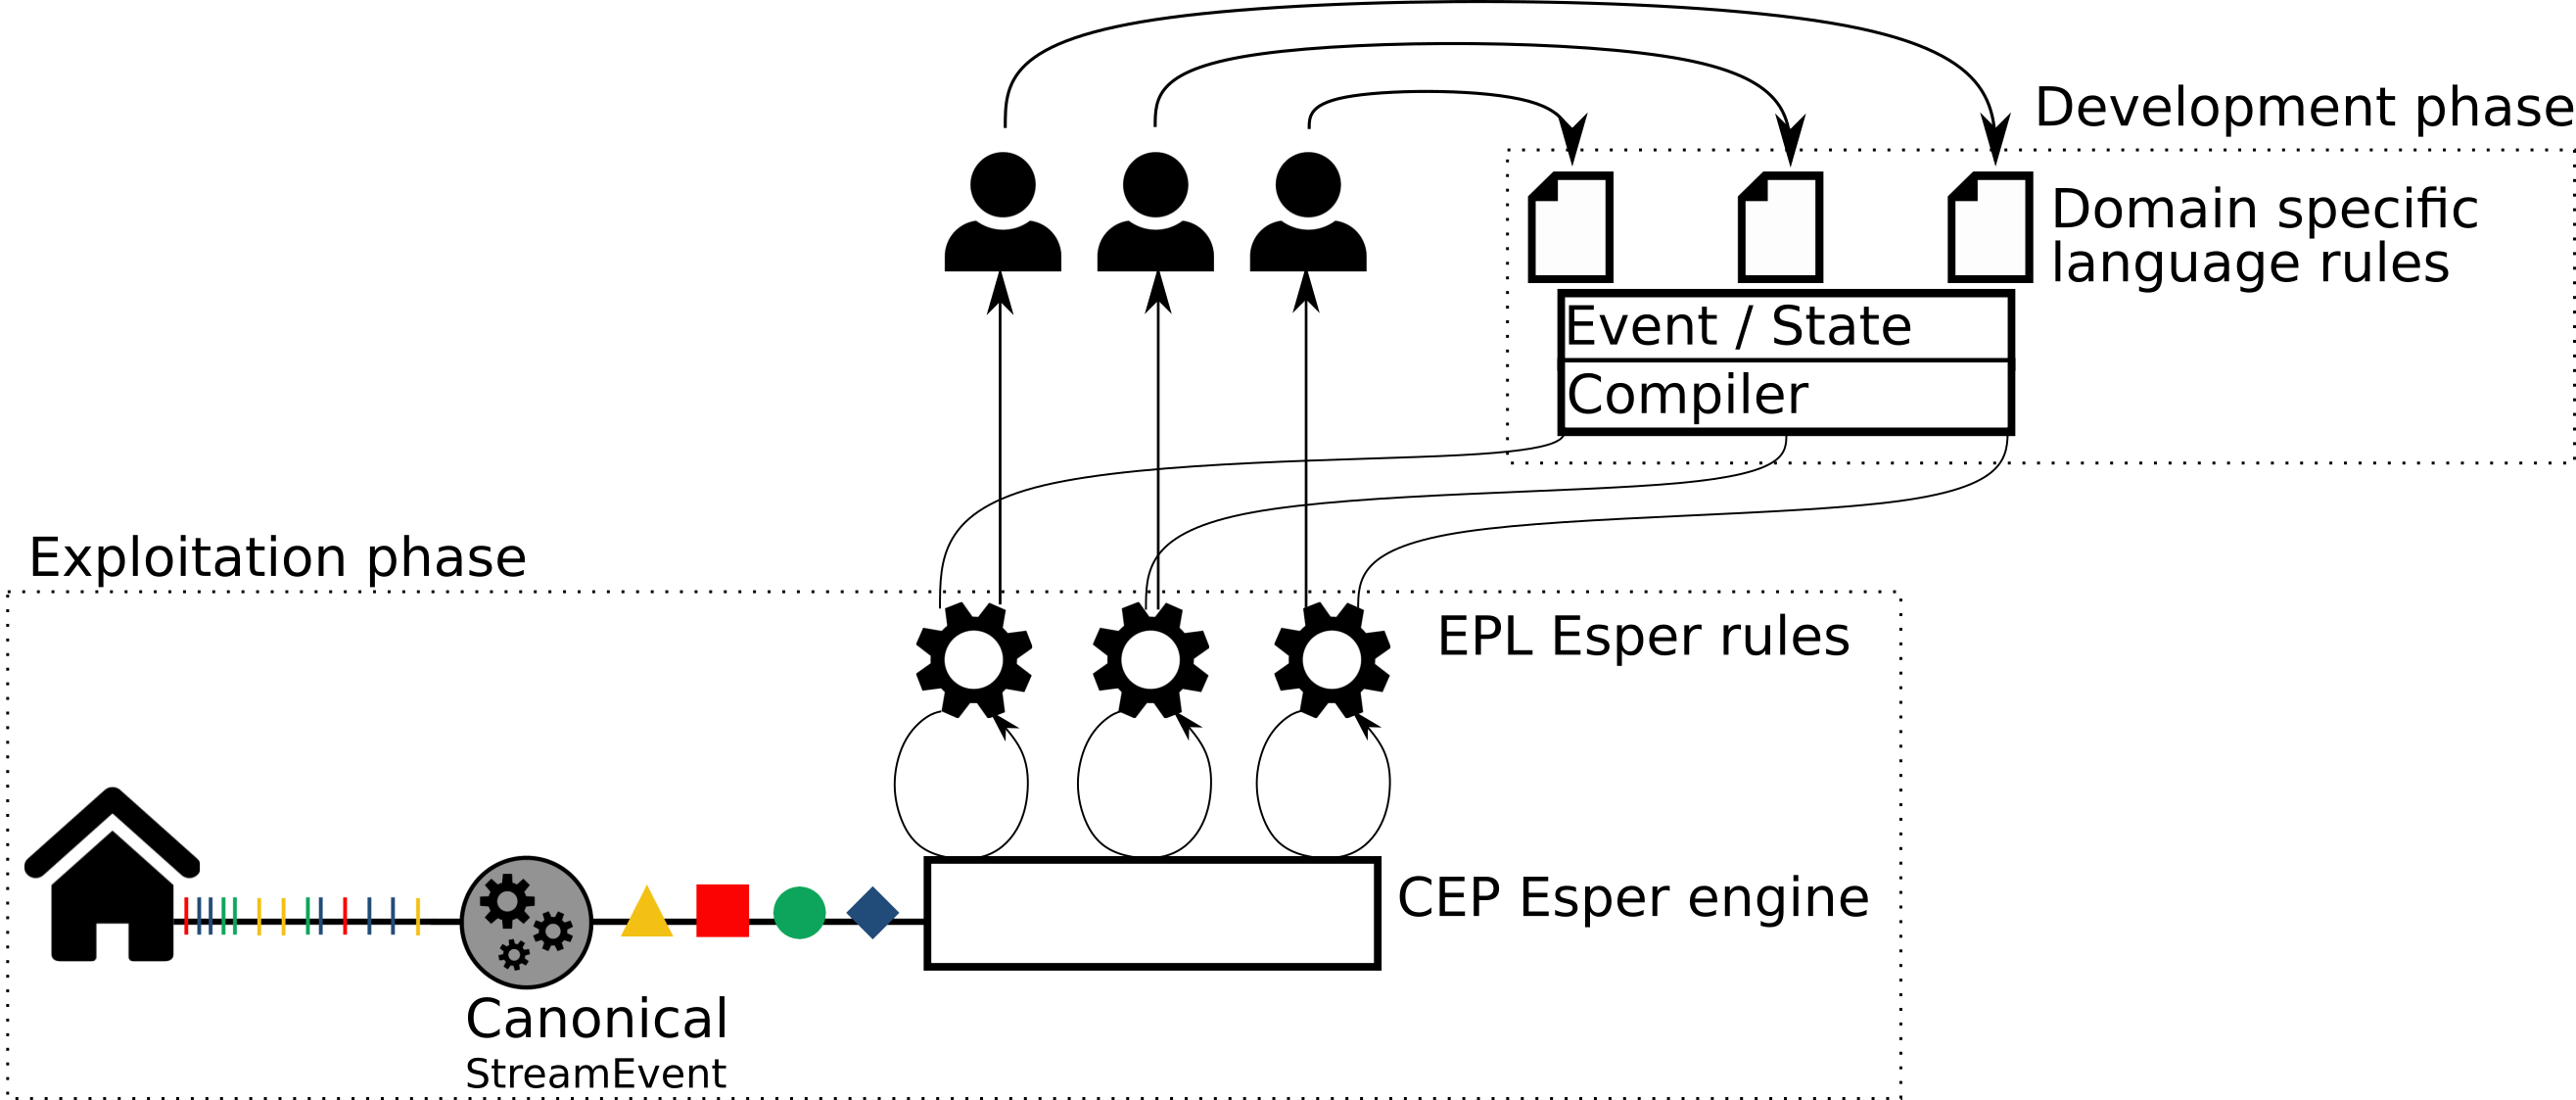
\includegraphics[scale=0.2]{gfx/approach}
\caption{Overall view of our domain-specific approach}
\label{fig:functionalarchi}
\end{figure}

\subsection{Définition du service}
La première étape est initiée avec les intervenants qui expriment les scénarios de services, comme illustré plus tôt. Ces scénarios sont directement écrit dans notre langage dédié par l'intervenant, si ils ont le bagage nécessaire ou par un développeur de services.

\subsection{Compilation du service}
Les services de haut niveau sont compilés dans des règles de plus bas niveau dans un langage de traitement d'évènement. Ces règles rendent explicite les concepts spécifiques au domaine, tels que les états qui sont compilés vers des combinaisons d'évènements et les opérations relatives.

\subsection{Exécution du service}
Pour être déployées, les règles sont ajoutés à un moteur de traitement d'évènement complexe (CEP). Notre moteur d'exécution de règle est basé sur Esper, un CEP open-source développé par EsperTech\footnote{http://www.espertech.com/esper/}. Esper propose des interface Java et C\# pour développer des programmes événementiels. Nous avons choisis Esper parce qu'il s'agit d'un moteur CRP populaire utilisé à la fois dans l'industrie et dans la recherche. Esper fournie un langage spécifique et déclaratif pour le traitement d'évènement complexes, appelé EPL (pour Event Processing Language). EPL permet de décrire des motifs d'évènements à identifier dans un flux d'évènements temps réel, en utilisant des opérateurs pour ordonner les évènements, des contraintes temporelles, {\em etc.} Esper ne permet pas de manipuler le concept d'état; il permet uniquement de traiter des évènements et nécessite donc quelques manipulations pour gérer un état. Dans notre implémentation, nous utilisons Esper avec règles EPL, compilées depuis des règles écrites en langage Maloya, et un flux d'évènement issue de domiciles sensibles au contexte, formattés en une forme canonique.

\subsection{Forme canonique}
La forme canonique de données produites par un domiciles sensibles au contexte permet de faire les traitement de façon uniforme, indépendemment de leur format hétérogène original. Dans notre implémetation, la forme canonique de données, appelée {\em StreamEvent}, est introduite comme couche d'abstraction sur le flux d'évènements de données. Dans cette représentation, chaque évènement est un 4-tuple du type d'évènements, sa localisation, sa valeur, et l'horodatage de son occurrence.

\section{Validation}\label{sec:validation}

Cette section présente la validation de notre approche sur la plate-forme DomAssist. L'expressivité de notre langage est validé en redéfinissant des services existant sur cette plate-forme. La justesse de notre compilateur est validée en comparant les résultats de l'exécution de nos règles compilées avec des services existants et déployés sur la plate-forme. Enfin, l'efficacité de notre langage est validé en mesurant certains les performances pertinentes pour le domaine de notre implémentation.

%\begin{landscape}
\begin{figure*}[h]
  \scriptsize
  \begin{tabular}{|l|p{7cm}|c|c|c|c|l|} 
    \hline
    \multirow{3}{*}{\textbf{Name}}&\multirow{3}{*}{\textbf{Description / DSL}}&\multicolumn{4}{|c|}{\textbf{Metrics}}&\multirow{3}{*}{\textbf{Stakeholders}}\\
    \cline{3-6}
                                  &                 &\multicolumn{2}{|c|}{\textbf{DSL}}&\multicolumn{2}{|c|}{\textbf{EPL}}&\\
                                  & & \# events & \# states & \# events & \# not &\\
    \hline
%**********************************************
    Presence & \cellcolor{gray!15}Detect if cupboard status changes while no presence in kitchen& \multirow{2}{*}{1}& \multirow{2}{*}{1} & \multirow{2}{*}{2}& \multirow{2}{*}{1} & Sensor\\ % \cline{2-2}
    dependency  & \begin{lstlisting}             
      Cupboard becomes open $\textbf{occurs}$ $\textbf{while}$ Presence(Kitchen) is false 
    \end{lstlisting} & & & && installer\\
    % &  & & && &\\
    % &  & & & &&\\
    \hline
%**********************************************
    Departure & \cellcolor{gray!15} Detect if entrance door is opened at least for 5 minutes during calendar night time & \multirow{4}{*}{1} & \multirow{4}{*}{1} & \multirow{4}{*}{2}& \multirow{4}{*}{2} & Occupational\\
                                 alert & \begin{lstlisting}  
                                    Door is open $\textbf{for}$ 5 minutes $\textbf{occurs}$ $\textbf{while}$ Night time
                                  \end{lstlisting} & & & &&  therapist \\ 
                                 &  & & & && Caregiver \\
    \hline
%**********************************************
    \multirow{2}{*}{Door alert} &\cellcolor{gray!15} Detect if entrance door is opened at least for 5 minutes during their is no presence in entrance& \multirow{4}{*}{0} & \multirow{4}{*}{2} & \multirow{4}{*}{4}& \multirow{4}{*}{6} &User \\
                                  & \begin{lstlisting}
                                    Door is open $\textbf{occurs}$ $\textbf{for}$ 5 min $\textbf{while}$ Presence(Entrance) is false
                                  \end{lstlisting} & &  && &  Caregiver \\
                                  &  & & && & \\
    \hline
%**********************************************
    Long &\cellcolor{gray!15} Detect if no movement in Bedroom since 24 hours & \multirow{3}{*}{0} &\multirow{3}{*}{1} & \multirow{3}{*}{1}& \multirow{3}{*}{1} & Occupational\\ %\cline{2-2}
    inactivity & \begin{lstlisting}
      Presence(Bedroom) is false $\textbf{for}$ 24 hours
    \end{lstlisting} & & & &&  therapist \\
                                  & & & & && Caregiver \\
    \hline
%**********************************************
    Fridge &\cellcolor{gray!15} Detect if fridge remains open at least 5 minutes &\multirow{2}{*}{0} &\multirow{2}{*}{1} & \multirow{2}{*}{1} & \multirow{2}{*}{1} & User\\% \cline{2-2}
    opened & \begin{lstlisting} 
      Fridge is open $\textbf{for}$ 5 minutes
    \end{lstlisting}& & & && Caregiver \\
    \hline
%********************************************** 
    \multirow{2}{*}{Breakfast} &\cellcolor{gray!15} Detect cupboard and coffeemaker opening (any order) during breakfast period & \multirow{3}{*}{2} & \multirow{3}{*}{1}&\multirow{3}{*}{3}&\multirow{3}{*}{1} & User\\% \cline{2-2}
                                  &  \begin{lstlisting} 
                                    $\textbf{\{}$Cupboard becomes open $\textbf{and}$ CoffeeMaker becomes on$\textbf{\}}$ 
                                    $\textbf{occurs}$ $\textbf{while}$ BreakfastTime 
                                  \end{lstlisting} & & & && Caregiver \\
    \hline
%**********************************************
    Lunch &\cellcolor{gray!15} Detect freezer opening and stove use in the 10 minutes following or freezer opening during stove use & \multirow{8}{*}{3} & \multirow{8}{*}{2} & \multirow{8}{*}{5}& \multirow{8}{*}{3} & Caregiver \\ %\cline{2-2}
    reheat &\cellcolor{gray!15} all during lunch period & & & & & User \\ %\cline{2-2}
     & \begin{lstlisting}  
      $\textbf{\{}$ ( Freezer becomes open $\textbf{precedes}$ $\textbf{within}$ 10 minutes 
          Stove becomes on ) 
        $\textbf{or}$ 
        ( Freezer becomes open $\textbf{occurs}$ $\textbf{while}$ 
          Stove is on ) $\textbf{\}}$
      $\textbf{occurs}$ $\textbf{while}$ Lunch Time
    \end{lstlisting}& & & & & \\                              
    \hline
%**********************************************
    \multirow{2}{*}{Dinner} & \cellcolor{gray!15} Detect fridge opening and microwave use (any order) during dinner period & \multirow{3}{*}{2} & \multirow{3}{*}{1} &\multirow{3}{*}{2} & \multirow{3}{*}{1} & User\\ %\cline{2-2}
                                  & \begin{lstlisting}  
                                    $\textbf{\{}$Fridge becomes open $\textbf{and}$ Microwave becomes on$\textbf{\}}$
                                    $\textbf{occurs}$ $\textbf{while}$ Dinner Time
                                   \end{lstlisting} & & & && Caregiver \\
    \hline
%**********************************************
    Go &\cellcolor{gray!15} Detect end of presence in bathroom and begin of presence in bedroom in the 10 minutes following & \multirow{5}{*}{2} & \multirow{5}{*}{1} & \multirow{5}{*}{3} & \multirow{5}{*}{2} &Caregiver \\ % \cline{2-2}
    to bed  &\cellcolor{gray!15} during go-to-bed period & & & & &User \\ 
    &  \begin{lstlisting} 
      ( Presence(Bathroom) becomes false $\textbf{precedes}$ $\textbf{within}$ 10 minutes 
        Presence(Bedroom) becomes true ) 
      $\textbf{occurs}$ $\textbf{while}$ Go-to-bed Time
    \end{lstlisting} & & & && \\
    \hline
%**********************************************
    \multirow{2}{*}{Wake-up} &\cellcolor{gray!15} Detect end of presence in bedroom and begin of presence in kitchen in the 10 minutes following & \multirow{5}{*}{2} & \multirow{5}{*}{1} & \multirow{5}{*}{3} & \multirow{5}{*}{2} & Caregiver \\ %\cline{2-2}
                                  &\cellcolor{gray!15} during go-to-bed period & & & & &User \\ 
                                  & \begin{lstlisting} 
                                    ( Presence(Bedroom) becomes false $\textbf{precedes}$ $\textbf{within}$ 10 minutes
                                      Presence(Kitchen) becomes true )
                                    $\textbf{occurs}$ $\textbf{while}$ Wake-up Time
                                  \end{lstlisting}& & & && \\
                                  % &  precedes within 10 min& & & && User\\
                                  % &  Presence(Kitchen) becomes true ) & & & && \\
                                  % &  occurs while Wake-up-time & & & && \\
    \hline
%**********************************************
    Commfailure &\cellcolor{gray!15} Detect any sensor that fails to communicate & \multirow{2}{*}{1} & \multirow{2}{*}{0} & \multirow{2}{*}{1} & \multirow{2}{*}{0} & Platform \\% \cline{2-2}
      warning& \begin{lstlisting}  
        Commfailure( Any ) becomes true 
        \end{lstlisting}& & & && maintainer \\
    \hline
%**********************************************
    Commfailure &\cellcolor{gray!15} Detect any sensor that has failed to communicate since 24 hours & \multirow{4}{*}{0} & \multirow{4}{*}{1} & \multirow{4}{*}{1} & \multirow{4}{*}{1} & Platform\\ %\cline{2-2}
      alert&  \begin{lstlisting} 
        Commfailure( Any ) is true $\textbf{for}$ 24 hours 
        \end{lstlisting}& & & &&  maintainer \\
                                  & & & & && Sensor \\
                                  & & & & && installer \\
    \hline
%**********************************************
    Battery & \cellcolor{gray!15} Detect battery level of any senser that become less than 5\% & \multirow{2}{*}{1} & \multirow{2}{*}{0} & \multirow{2}{*}{1} & \multirow{2}{*}{0} & Sensor\\ %\cline{2-2}
    alert & \begin{lstlisting}
      BatteryLevel( Any ) becomes $\textit{less than}$ 5 
      \end{lstlisting}& & & && installer\\
    \hline
  \end{tabular}
  \caption{Services examples}
  \label{app_examples}
\end{figure*}
%\end{landscape}

\subsection{Expressivité}\label{validation:expressiveness}
Pour validé l'expressivité de notre langage, nous avons réimplanté 55 services déjà déployés dans DomAssist. Ces services sont les variation des 13 familles de règles listés en Figure~\ref{app_examples}. Des variations sont requises pour satisfaire les spécificités des personnes âgées. Par exemples, la détection des activités du quotidien comme la préparation du repas et le lever/coucher, doit être personnalisée pour chaque utilisateur dans le respect des capacités de mesures des interactions l'environnement, périodes de reconnaissance des activités, et des périodes de temps entre les séquences d'intéractions. Par exemple, pour préparer le petit déjeuner, une personne âgée peut utiliser un presse agrume électrique et prendre un verre dans un placard spécifique, alors qu'un autre peut utiliser une bouilloire et ouvrir le frigidaire our prendre du lait.

Réécrire une éventail de service nous permet de valider que notre langage et ses concepts sous-jacents (évènements, états, opérateurs d'Allen) sont suffisamment expressif pour couvrir des cas réels de services dans le domaine du maintien à domicile de personnes âgées.

%\subsection{Compilation}\label{validation:compilation}
\subsection{Exactitude}\label{validation:results}
%We did not attempt to prove the correctness of our DSL compiler with respect to a formal semantics of its operators, although this work would be of interest. Instead, we empirically validated the correctness of the compiled services by a combination of visual code inspection and extensive testing. We performed manual inspection of all the intermediate forms described earlier (core DSL, EPL pseudo-code, Esper EPL) to ensure that they remain consistent with their original counterparts.

Nous avons validé empiriquement l'exactitude de nos services compilé par des inspections visuels et des tests étendu. Nous avons inspecté manuellement les formes intermédiaires décrites précédemment (pseudo-code EPL, EPL Esper) pour nous assurer de la cohérence des résultats des différentes étapes de compilation.

Ensuite, nous avons validé la sortie du compilateur ({\em i.e.,} règle EPL résultante) en deux phases. Premièrement, nous avons testé les règles en les exécutant sur des fichiers de logs provenant du projet DomAssist. Ces logs contiennent des évènements horodatés produits par tous les capteurs de l'infrastructure, qu'ils soient matériels ou logiciels. Les résultats ont été automatiquement vérifié par des scripts Perl, implantant les même spécifications de service. Ces scripts sont plus simple à écrire que les vrais applications puisqu'ils exécutent les logs de données, ils n'ont ainsi pas à traiter les résultats en temps réel, et n'ont pas à traiter avec l'infrastructure de capteurs.

%We repeatedly compared the results produced by the compiled DSL services and the scripted specifications on extended log histories. This iterative process allowed us to refine our compilation schemas until it produced the same results as the scripted specifications.

Dans une seconde phase, nous avons connecté nos services au flux d'évènements temps réel sur la plate-forme de production pour neuf utilisateurs pendant un mois, en parallèle des services existants écrits en Java. Aucune différences n'ont été observées dans les résultats entre les deux systèmes (Java et règles compilées depuis notre langage). De plus cette phase nous à permis d'évaluer les performances à l'exécution de notre approche.


\subsection{Performances}\label{validation:performance}
Pour valider l'utilisabilité de notre approche à base de langage dédié en pratique, nous avons mesuré en conditions réelles, les performances des règles EPL produites par notre compilateur avec deux indicateurs: la latence de détection, et la consommation mémoire de notre moteur d'exécution. Les règles sont exécutées sur notre serveur de production (quad-core Intel(R) Xeon(R) E5-2407 v2 2.4 GHz CPU et 125GB RAM).

La latence de détection d'une règle donne le temps entre le dernier évènement qui déclenche une règle, et sont déclanchement effectif. Une latence faible indique que la règle est suffisamment réactive pour un usage pratique. D'après nos mesures, cette latence pour nos règles est toujours inférieur à une seconde. Cet ordre de grandeur est parfaitement compatible avec le type de règle qui sont implanté dans la plate-forme pour le maintien à domicile des personnes âgées.

Nous avons également mesuré la consommation mémoire de notre implémentation pour nous assurer qu'elle peut passer à l'échelle pour des centaines d'utilisateurs et des dizaines de services. D'après nos mesures, la consommation mémoire est de 352MB en moyenne pour 55 règles, traitant les données de 129 domiciles pendant un mois 24 heures sur 24. Encouragés par ces résultats, nous avons entrepris d'explorer la possibilité d'appliquer notre approche et notre implantation sur une architecture plus limitée, mais plus accessible et fréquemment utilisée en informatique ubiquitaire, un Raspberry Pi 3 (quad-core ARM Cortex-A53 1.2 GHz CPU et 1GB RAM). Durant cette expérimentation, nous avons exécuté les même 55 règles avec les mêmes 129 installations pendant un mois. La consommation mémoire constatée est de 173MB en moyenne. Cette moindre consommation mémoire sur le Raspberry Pi s'explique par son architecture 32-bit.
Ces mesures nous montre que notre apporche est applicable tant sur une infrastructure cloud que sur une infrastructure embarquée directement à l'intérieur du domicile.

\section{Discussion}

Our DSL bridges the gap between high-level domain concepts and low-level mechanisms of event handling. As a consequence, it contributes to making rules more concise and  to simplify their development, by encapsulating details of event handling in a compiler.  Indeed, the original Java applications implementing HomeAssist services contain manually implemented timed automata, which recognize the sequences of events corresponding to each DSL rule.  Timing constraints are explicitly handled by using a timer service, producing timeout events that are inserted in the stream of events, produced by the sensor infrastructure.  In our DSL rules, these low-level details of state and time handling are included in the semantics of operators.  For instance, the role of explicit timers corresponds the parameters of our time-constrained operator variants. This lowers the efforts to write rules and to make them more predictable.

\subsection*{Limitations}

Our approach is a first step towards simplifying the development of context-aware applications in the domain of aging in place, and presents a number of limitations.

First of all, our DSL only is dedicated to recognizing contexts. It provides no constructs for performing actions on the environment. These must be currently programmed in a generic programming language. It would be useful to extend our domain analysis to also cover the control part of typical applications, and to derive domain-specific concepts and notations to perform actions.

As far as applications are concerned, we have designed and tested our DSL only on services in the domain of aging in place, which involves a specific set of composition operators. However, our DSL can express rich, arbitrarily nested combinations. It would be interesting to apply it to other domains of context-aware applications in the future.

Finally, our rules always return boolean values. However, context-aware information may sometimes be more general than strictly binary. For instance, a daily activity such as meal preparation might be detected in a more nuanced way as a probability between 0 and 1, to cope with some amount of deviations from the user's routine. Currently, in our DSL the different routine variations must be coded as different rules, which is not always practical. In the future, it would be interesting to consider extending our approach with operators returning non-boolean values.
% Such fuzzy detectors are sometimes used in the domain of aging in place.

\section{Conclusion}
%**********************************************
%**********************************************

We have proposed a new approach for developing context-aware services in a smart home, by
analyzing a range of existing data processing layers in the domain of aging in place. We have identified key concepts and operations specific to context-aware processing. Based on this analysis, we have introduced a context-aware, domain-specific language and its software architecture, which allow to put in synergy the stakeholders of a context-aware home by providing them with a unified approach to designing and developing services. Our approach offers context aware-specific abstractions and notations, within a data-centric and data-driven paradigm.

We have validated our approach by applying it to an assisted living platform for aging in place. In particular, we have used our domain-specific language to re-implement existing services of the assisted living platform. These services were deployed and successfully tested for their effectiveness in performing the specific tasks of the stakeholders: detection of daily activities, detection of user risks, sensor failure, {\em etc.}
